\documentclass[12pt,a4paper]{article}
\usepackage[margin=2cm]{geometry}
\usepackage{titling}
\usepackage{graphicx}
\usepackage{subcaption}
\setlength{\droptitle}{-5em} 
\usepackage{algorithm} 
\usepackage{algpseudocode}
\usepackage{enumerate}
\usepackage{float}


\begin{document}
\title{\huge \textbf{Overall Software Plan} \\ \LARGE {\textbf{CS 346: Assignment-2A}}}
\author{\Large Academic Section Management Software}
\date{Group 10A : \texttt{210101113-210101119}}
\maketitle


\section{Problem Statement and Stakeholders}
(Yashraj)

\section{Software Model}
The adoption of the \textbf{Structured Analysis and Design} (SAD) model for the development of this specific software is justified by the intricate design and the comprehensive requirements that demand careful consideration. This report documents the different components of this model, including the \textit{Data Dictionary} (encompassing Requirements and Assumptions), \textit{Data Flow Diagrams} (DFDs), and \textit{Entity-Relationship} (E-R) Diagrams in the following sections below.
    
\section{Software Requirements and Assumptions}
The following are the specifications of the software that has to be developed that has been mentioned in the problem statement: (Agrawal)
\begin{itemize}
    \item Item1
    \item Item2
\end{itemize}

\section{Data Flow Diagrams}
Short Desc (Yashraj) \textbf{Bold}, \texttt{Verb}, \textit{Italics}
\subsection{Level-0 DFD}
(Yashraj)
\subsection{Level-1 DFD}
(Yashraj)

\subsection{Level-2 DFDs}
The following subsections highlight the detailed \textbf{Level-2} Dataflow diagrams of various processes in the Academic system Management software:
\subsubsection{Admission Management Module}
(Gupta)
\subsubsection{Course Management Module}
(Tanish)
\subsubsection{Examination Management Module}
(Pratyush)
\subsubsection{Grade Management Module}
\begin{figure}[hbt!]
    \centering
        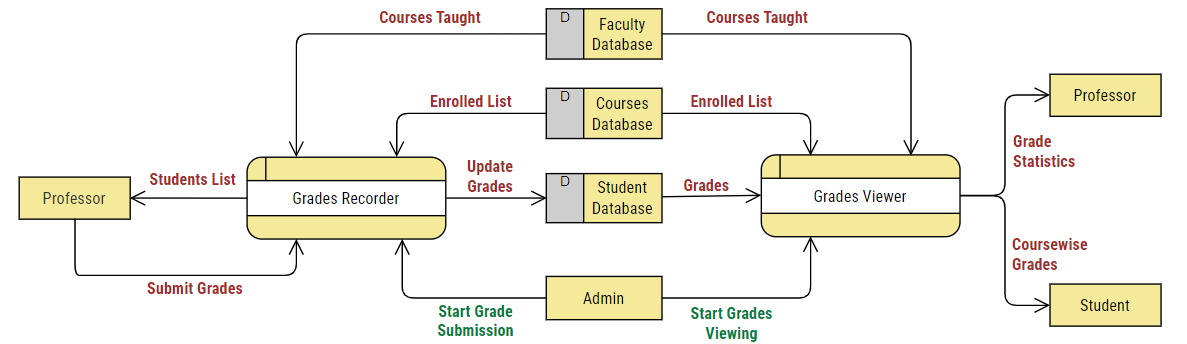
\includegraphics[width=\linewidth]{Grade_Management_DFD.png} 
    \caption{Level-2 DFD of Grade Management Module}
\end{figure}
\begin{itemize}
    \item The \textbf{Grade Recorder} Process first gets the signal from the Admin side to start grade submission.
    \item The professors are displayed the various courses that they teach and they can upload the grade list of students enrolled coursewise, which are updated duly by the Grade Recorder process into \texttt{Grades} field of each course taken by student in \textbf{Student Database}.
    \item The \textbf{Grades Viewer} process first gets the signal from the Admin side after which the students are displayed the grades that they got in specific courses.
    \item The professors can get overall statistics about the grades like Class Average,number of students who got different grades like \texttt{AA,AB,BB} etc.
    \item This particular module interacts with the databases to fetch and update the results, as shown in the DFD diagram of Grade Management module.
\end{itemize}
\section{Entity Relationship Diagram}
    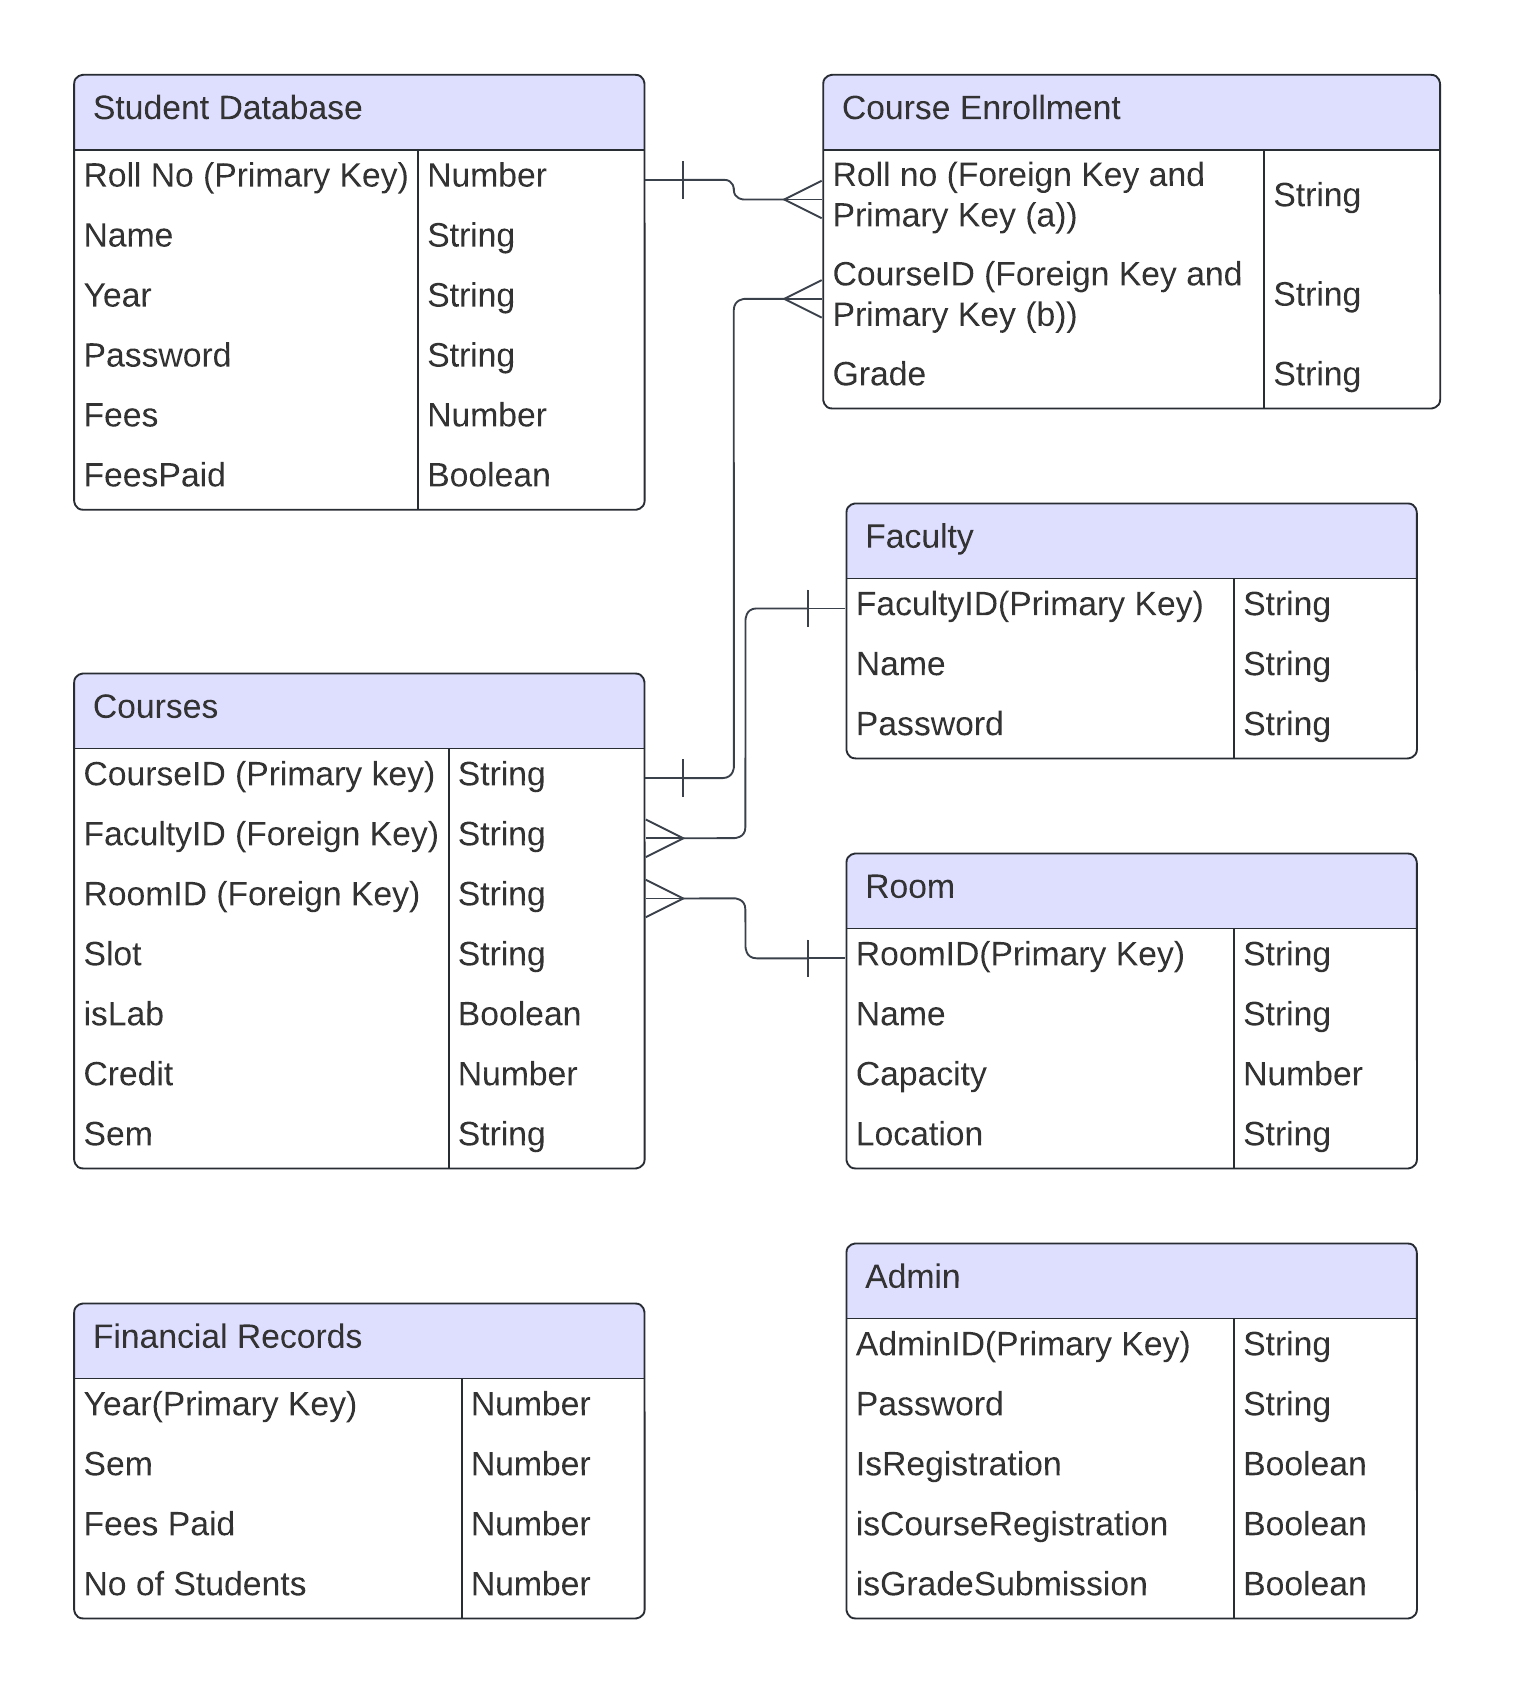
\includegraphics[scale=1.2]{ERDiagram.png}

    Each Arrow represents a relation. A multiple-forked arrow represents Many relationships, whereas a single bar arrow represents one
    
    
    \subsection{Student Database}
        This database is used to store all information regarding students. The description of Each key is as follows:
        \begin{itemize}
        \item \textbf{Roll No:} Roll Number of student serves as Primary Key
        \item  \textbf{Name:} Name of Student
        \item  \textbf{Year:} Year Of Joining
        \item  \textbf{Password:} Password Used for authentication Purposes
        \item  \textbf{Fees:} Amount to be Paid By student
        \item  \textbf{FeesPaid:} Boolean to store if Fees paid or not
    \end{itemize}
    \subsection{Courses Database}
        This database is used to store all information regarding Courses.  The description of Each key is as follows:
        \begin{itemize}
        \item \textbf{CourseID:} Unique Identifier for Each Course. Serves as Primary key.
        \item  \textbf{FacultyID:} ID of faculty taking this course serves as a Foreign Key to faculty Table.
        \item  \textbf{RoomID:} ID of Room where this course will be held serves as a Foreign Key to Room Database.
        \item  \textbf{Slot:} Slot in which this course lectures are held. Assigned by TimeTable generator.
        \item  \textbf{isLab:} Boolean to store if It is a lab or not.
        \item  \textbf{Credit:} Credits of this course.
        \item  \textbf{Sem:} String to store sems in which this course is offered.
    \end{itemize}
    \subsection{Courses Taken Database}
        This database is used to store all information regarding which student took which Course. The pair (Roll No, CourseID) serves as a Primary Key. The description of Each key is as follows:
        \begin{itemize}
        \item \textbf{Roll No:} Roll No of student who has taken this course. Serves as Foreign Key to student Database.
        \item  \textbf{CourseID:} ID of Course taken. Serves as a Foreign Key to Courses Table.
        \item  \textbf{Grade:} Grade Received by student in that particular Course
    \end{itemize}
    \subsection{Faculty Database}
        This database is used to store all information regarding Faculties.  The description of Each key is as follows:
        \begin{itemize}
       \item \textbf{FacultyID:} Unique Identifier for Each Faculty. Serves as Primary key.
        \item  \textbf{Name:} Name of Faculty
        \item  \textbf{Password:} Password Used for authentication Purposes
    \end{itemize}
     \subsection{Room Database}
        This database is used to store all information regarding Rooms. The description of Each key is as follows:
        \begin{itemize}
       \item \textbf{RoomID:} Unique Identifier for Each Room. Serves as Primary key.
        \item  \textbf{Name:} Name of Room
        \item  \textbf{Capacity:} Capacity of Room
        \item  \textbf{Location:} Location of Room
    \end{itemize}
    \subsection{Admin Database}
        This database is used to store all information regarding Admin who controls the system. The description of Each key is as follows:
        \begin{itemize}
       \item \textbf{AdminID:} Unique Identifier for Admins. Serves as Primary key.
        \item  \textbf{Password:} Password Used for authentication Purposes
        \item  \textbf{isRegistration:} Boolean to start admission and Registration of new students.
        \item  \textbf{isCourseRegistration:} Boolean to start course Registration.
        \item  \textbf{isGradeSubmission:} Boolean to start Grade Submission.
    \end{itemize}
    \subsection{Financial Records}
        This database is used to store all information related to Finances. The description of Each key is as follows:
        \begin{itemize}
       \item \textbf{Year:} Year of Financial Record. Serves as Primary key.
        \item  \textbf{Sem:} Semester
        \item  \textbf{FeesPaid:} How much Fees is paid.
        \item  \textbf{No of Students:} Number of Registered Students.
    \end{itemize}
\section{Feature Enhancement}
(Shivam)
\begin{itemize}
    \item hrtrt
    \item rtrtrtrttrt
\end{itemize}
        
\section{User Interface}
(Shivam Agrawal)
	The user interface for this software can be developed using \texttt{Visual Basic}. The following are the tentative list of toolbox components needed for the basic implementation (without any feature enhancement):
    \begin{itemize}
        \item \textbf{Text Box:} sdfeerererererer
        \item And so on....
    \end{itemize}

    \subsection{Basic Design}
    This is the tentative basic design of the user interface which is to be designed in \textbf{Visual Basic} using the components listed above:
    \begin{figure}[h]
        \centering
        \begin{subfigure}[b]{0.45\linewidth}
            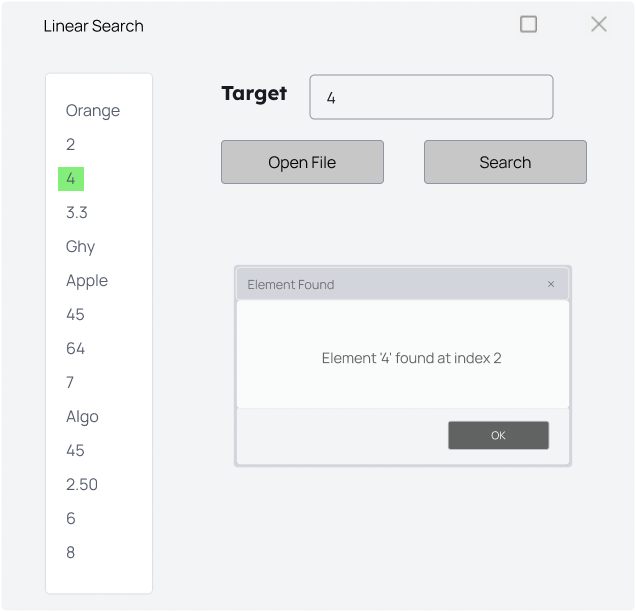
\includegraphics[width=\linewidth]{Prototype.png} 
            \caption{Message box output when element is found.}
            \label{fig:sub1}
        \end{subfigure}
        \hfill
        \begin{subfigure}[b]{0.45\linewidth}
            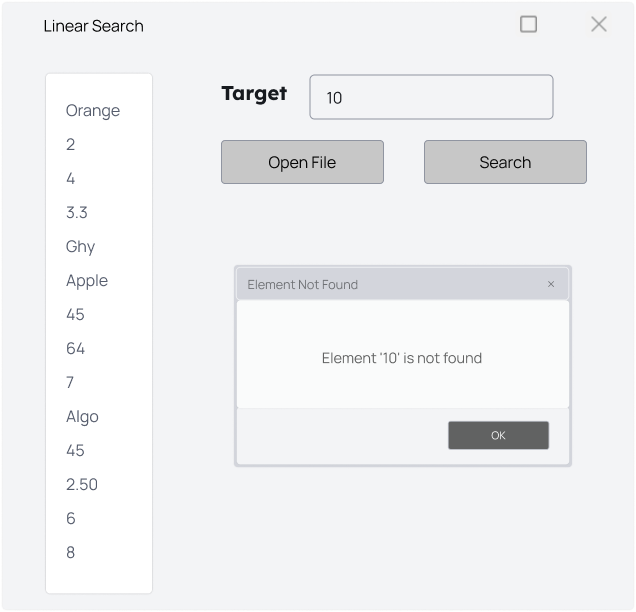
\includegraphics[width=\linewidth]{Prototype-2.png}
            \caption{Message box output when element is not found.}
            \label{fig:sub2}
        \end{subfigure}
        \caption{Basic design of the software application}
        \label{fig:overall}
    \end{figure}
\subsection{Subsections}
\end{document}